\chapter{Methodology}
%%WHAT Is inference3
\label{chap:methodology}
In this section a performance model, characterising the deployment of deep learning models for inference, is presented. To understand these characteristics, the underlying factors that affect it need to be understood first. Therefore we first describe the problem space before we can map the problem space on the performance model.


\section{Problem Space}
The inference performance of a deep learning model is mainly affected by three factors, the architecture of the model itself and the hardware environment where it gets deployed and the framework performing the operations of the model on the hardware environment.
These three aspect are covered in this section.


\subsection{Deep Learning}
%%Bisschen genauer was deep learning input output...
%Einfluss auf inference latency an memory?

Deep learning models are neural networks with many hidden layers and hidden units leading to deep architectures.
These deep architectures with often millions of parameters lead to a significant increase in computational power for both training and inference,
%While for simple linear regression model with a single variable a single computation

These models often have single input and output layer and in between the hidden layers containing the hidden units.

%the most popular being convolutional neural networks and recurrent neural networks right now, which are special forms of neural networks.
There are many different operators and network architectures, which makes performance prediction very complex.

%This increased amount of layers leads to complex mathematical calculations.
\begin{comment}
\subsubsection{Architectures}
\begin{itemize}
    \item layer
    \item hidden units
    \item input size
    \item number of operations
\end{itemize}
\end{comment}

\paragraph{Convolutional Neural Network}
This specific class of neural network achieved wide success in the field of image classification and detection in images. Convolutional Neural Networks (CNN) are used to extract features like complex shapes or colour patterns from images to perform image classification. Image classification network classify the contents of a image by outputting a class for the image with a respective confidence level, for example how likely an animal on a picture represents a cat.

This feature extraction is done with the use of convolutional and pooling layers. These layer types

%%bild mit simpler architecture? Bild->conv->pool->flatten->dense-> output


These deep architectures lead a high number of operations and parameters, resulting in high demands of computational power.
\subsubsection{Training}
After constructing the architecture of a model it can be trained to reach the highest accuracy using a data set. This data set consists of 
%forward and backprop
\subsubsection{Inference}
%only forward prop

After the model is trained it is ready to be deployed in a production environment, where it can serve its predictions to a an application. This process of feeding input data to a neural network, performing all computational operations defined in the model resulting in an output/prediction, is called inference.

But since models often require the input to be of a certain shape and the input given by an application often does not match that shape, a preprocessing step is often needed before the actual inference can be performed.
This preprocessing and inference process can also be seen in figure \ref{fig:InfProcess}.
%%Add visualization of input here
%%die dann im deployment wieder aufgreifen
\begin{figure}[H]
\centering


\tikzset{every picture/.style={line width=0.75pt}} %set default line width to 0.75pt        

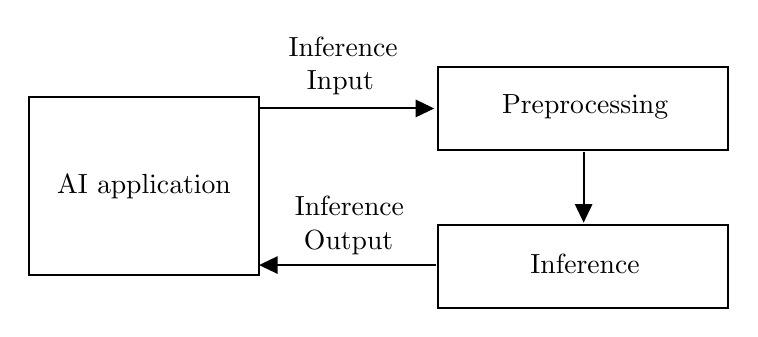
\begin{tikzpicture}[x=0.75pt,y=0.75pt,yscale=-1,xscale=1]
%uncomment if require: \path (0,300); %set diagram left start at 0, and has height of 300

%Shape: Rectangle [id:dp7725979857917211] 
\draw  [fill={rgb, 255:red, 255; green, 255; blue, 255 }  ,fill opacity=1 ] (262,80) -- (402,80) -- (402,120) -- (262,120) -- cycle ;
%Shape: Rectangle [id:dp3208391580840302] 
\draw  [fill={rgb, 255:red, 255; green, 255; blue, 255 }  ,fill opacity=1 ] (262,156) -- (402,156) -- (402,196) -- (262,196) -- cycle ;
%Straight Lines [id:da5532652572924177] 
\draw    (175.93,99.98) -- (258.29,99.98) ;
\draw [shift={(260.29,99.98)}, rotate = 180] [fill={rgb, 255:red, 0; green, 0; blue, 0 }  ][line width=0.75]  [draw opacity=0] (8.93,-4.29) -- (0,0) -- (8.93,4.29) -- cycle    ;

%Straight Lines [id:da9616587358279531] 
\draw    (332.29,121) -- (332.29,152.98) ;
\draw [shift={(332.29,154.98)}, rotate = 270] [fill={rgb, 255:red, 0; green, 0; blue, 0 }  ][line width=0.75]  [draw opacity=0] (8.93,-4.29) -- (0,0) -- (8.93,4.29) -- cycle    ;

%Straight Lines [id:da0888724954521467] 
\draw    (260.93,175.43) -- (177.93,175.43) ;
\draw [shift={(175.93,175.43)}, rotate = 360] [fill={rgb, 255:red, 0; green, 0; blue, 0 }  ][line width=0.75]  [draw opacity=0] (8.93,-4.29) -- (0,0) -- (8.93,4.29) -- cycle    ;

%Shape: Rectangle [id:dp6392688617606377] 
\draw  [fill={rgb, 255:red, 255; green, 255; blue, 255 }  ,fill opacity=1 ] (64.93,94.43) -- (175.93,94.43) -- (175.93,180.43) -- (64.93,180.43) -- cycle ;

% Text Node
\draw (333,99) node  [align=left] {Preprocessing};
% Text Node
\draw (333,175) node  [align=left] {Inference};
% Text Node
\draw (120.43,137.43) node  [align=left] {AI application};
% Text Node
\draw (216.43,79.43) node  [align=left] {Inference\\ \ \ Input};
% Text Node
\draw (219.43,156.43) node  [align=left] {Inference\\ \ Output};


\end{tikzpicture}
\caption{Visualisation of the inference process including preprocessing}
\label{fig:InfProcess}
\end{figure}
Note that the architecture of the inference model is often slightly different from the training model, as some operators are only needed for the training process and are thus removed for inference (e.\,g. dropout).






\subsubsection{Quantization}
\label{chap:quant}
Quantization is a technique that trades in model precision for better inference latencies, memory consumption during inference and model sizes.
Quantization describes the process of reducing the "precision representations of weights and, optionally, activations" \cite{tfLiteQuant} from floating point precision to for example 8-bit.
The weights/activations are either quantized after training the model with floats (Post Training Quantization) or the model is training with quantized weights/activations from the start (Quantization Aware Training). In the paper "Quantizing deep convolutional networks for
efficient inference"\cite{Quantizing} Krishnamoorthi performed a study on these technique with the following results:
8-bit quantization can lead to a model size reduction by a factor of 4, a 2x-3x latency speedup on CPUs and DSPs, while reducing the model accuracies by 1\%.


\subsection{Deployment of Deep Learning Models}
Deep learning deployment describes the process of deploying a trained machine learning model to a production environment for inference purposes. 

%%Write more here
There can be differentiated in two different deployment methods, the first one is deploying the model directly to edge devices, while the second outsources the model to a cloud-backend, where the inference is performed and the prediction is sent back to the edge device.
\subsubsection{Edge Deployment}
Edge devices are characterised by offering a limited amount of hardware specifications such as amount of available energy, memory and overall computational power.
These devices are often mobile devices like smartphones, cars or Raspberry Pis.
Despite its limits, edge deployment also has some advantages, particular in reliability and security. 
For example in the case of image classification images are needed for the inference, which often contain sensible information and thus raise a data privacy/security concern.
Therefore edge deployment is preferred, if the inference performance is sufficient for the use case of real time AI applications.

In order to increase this performance various accelerators like better GPUs, TPUs or other dedicated neural network hardware components have been developed for edge devices.

%% hier retrainign ansprechen; herausforderungen bei edge deployment (retrainign noch mehr computational intensive -> cloud rettraining and then redeployment on edge)
%viele edge geräte


\subsubsection{Cloud Deployment}
While the breakthroughs in deep learning are very interesting for AI applications on edge devices, the computational demand needed for edge deployment often exceeds the available power to be viable.
That is why the option of outsourcing the models to a cloud-backend has become a popular solution in the recent years.
Cloud-backends offer a huge amount of computational power, especially suitable for deep learning in the form of GPUs, TPUs, etc.


The big downside of cloud-based inference is the needed network connection, in particular for edge devices such as cars, where a reliable network connection can often not be guaranteed for example in rural areas. Hence this is not a viable solution for applications that are critical like autonomous driving.

While for the edge deployment necessary preprocessing steps are always done on the edge, for the case of cloud inference there a two possibilities. Either the input data is preprocessed to the correct shape before getting sent to the cloud-backend, or the input is sent unpreprocessed to the cloud. 
In the latter case the input gets preprocessed on the cloud. 
This can be justified by the same reasons as for the cloud inference, more computational power for intensive preprocessing.



\subsection{Deep Learning Inference Framework}
For both edge and cloud inference the underlying inference framework is important for the inference performance, since optimised kernels/operators or support of accelerators like GPUs can lead to significant performance improvements.
The framework needs to support the model operations as well as the hardware components to achieve a good performance.

%cloud inference network protocol

This is especially important for edge devices, where new accelerators are being developed at a fast pace.


%%
After analysing the problem space of deep learning inference for real-time AI applications on edge devices we can propose a performance model, that maps the aspects of the problem space on the performance.



\section{Performance Model}
All the aspects of hardware, model and the used inference framework have an impact on the performance, thus are the influencing factors of the performance model (see figure \ref{fig:perfmodel}). These inputs affect various performance metrics, of which inference latency and throughput are the most important ones for real-time AI applications. However, as the hardware on edge devices is limited and most of the times many applications need to run in parallel, low usages of the other depicted metrics are vital as well.
Except the data consumption, all metrics are relevant for both edge and cloud inference.
While accuracy is one of the most critical metrics for neural networks, it is only affected by the characteristics of the model and not by the deployment environment. Therefore we do not focus on accuracy in this thesis.

To get the model output for a given model input two steps are needed. The first one is the preprocessing step and transforms a given input into the format that is required by the deep learning model. Only then the actual inference operation can be performed to obtain the model output. Therefore the preprocessing takes a vital part in the general inference process and should be included in the performance model.
\begin{figure}[H]
\centering
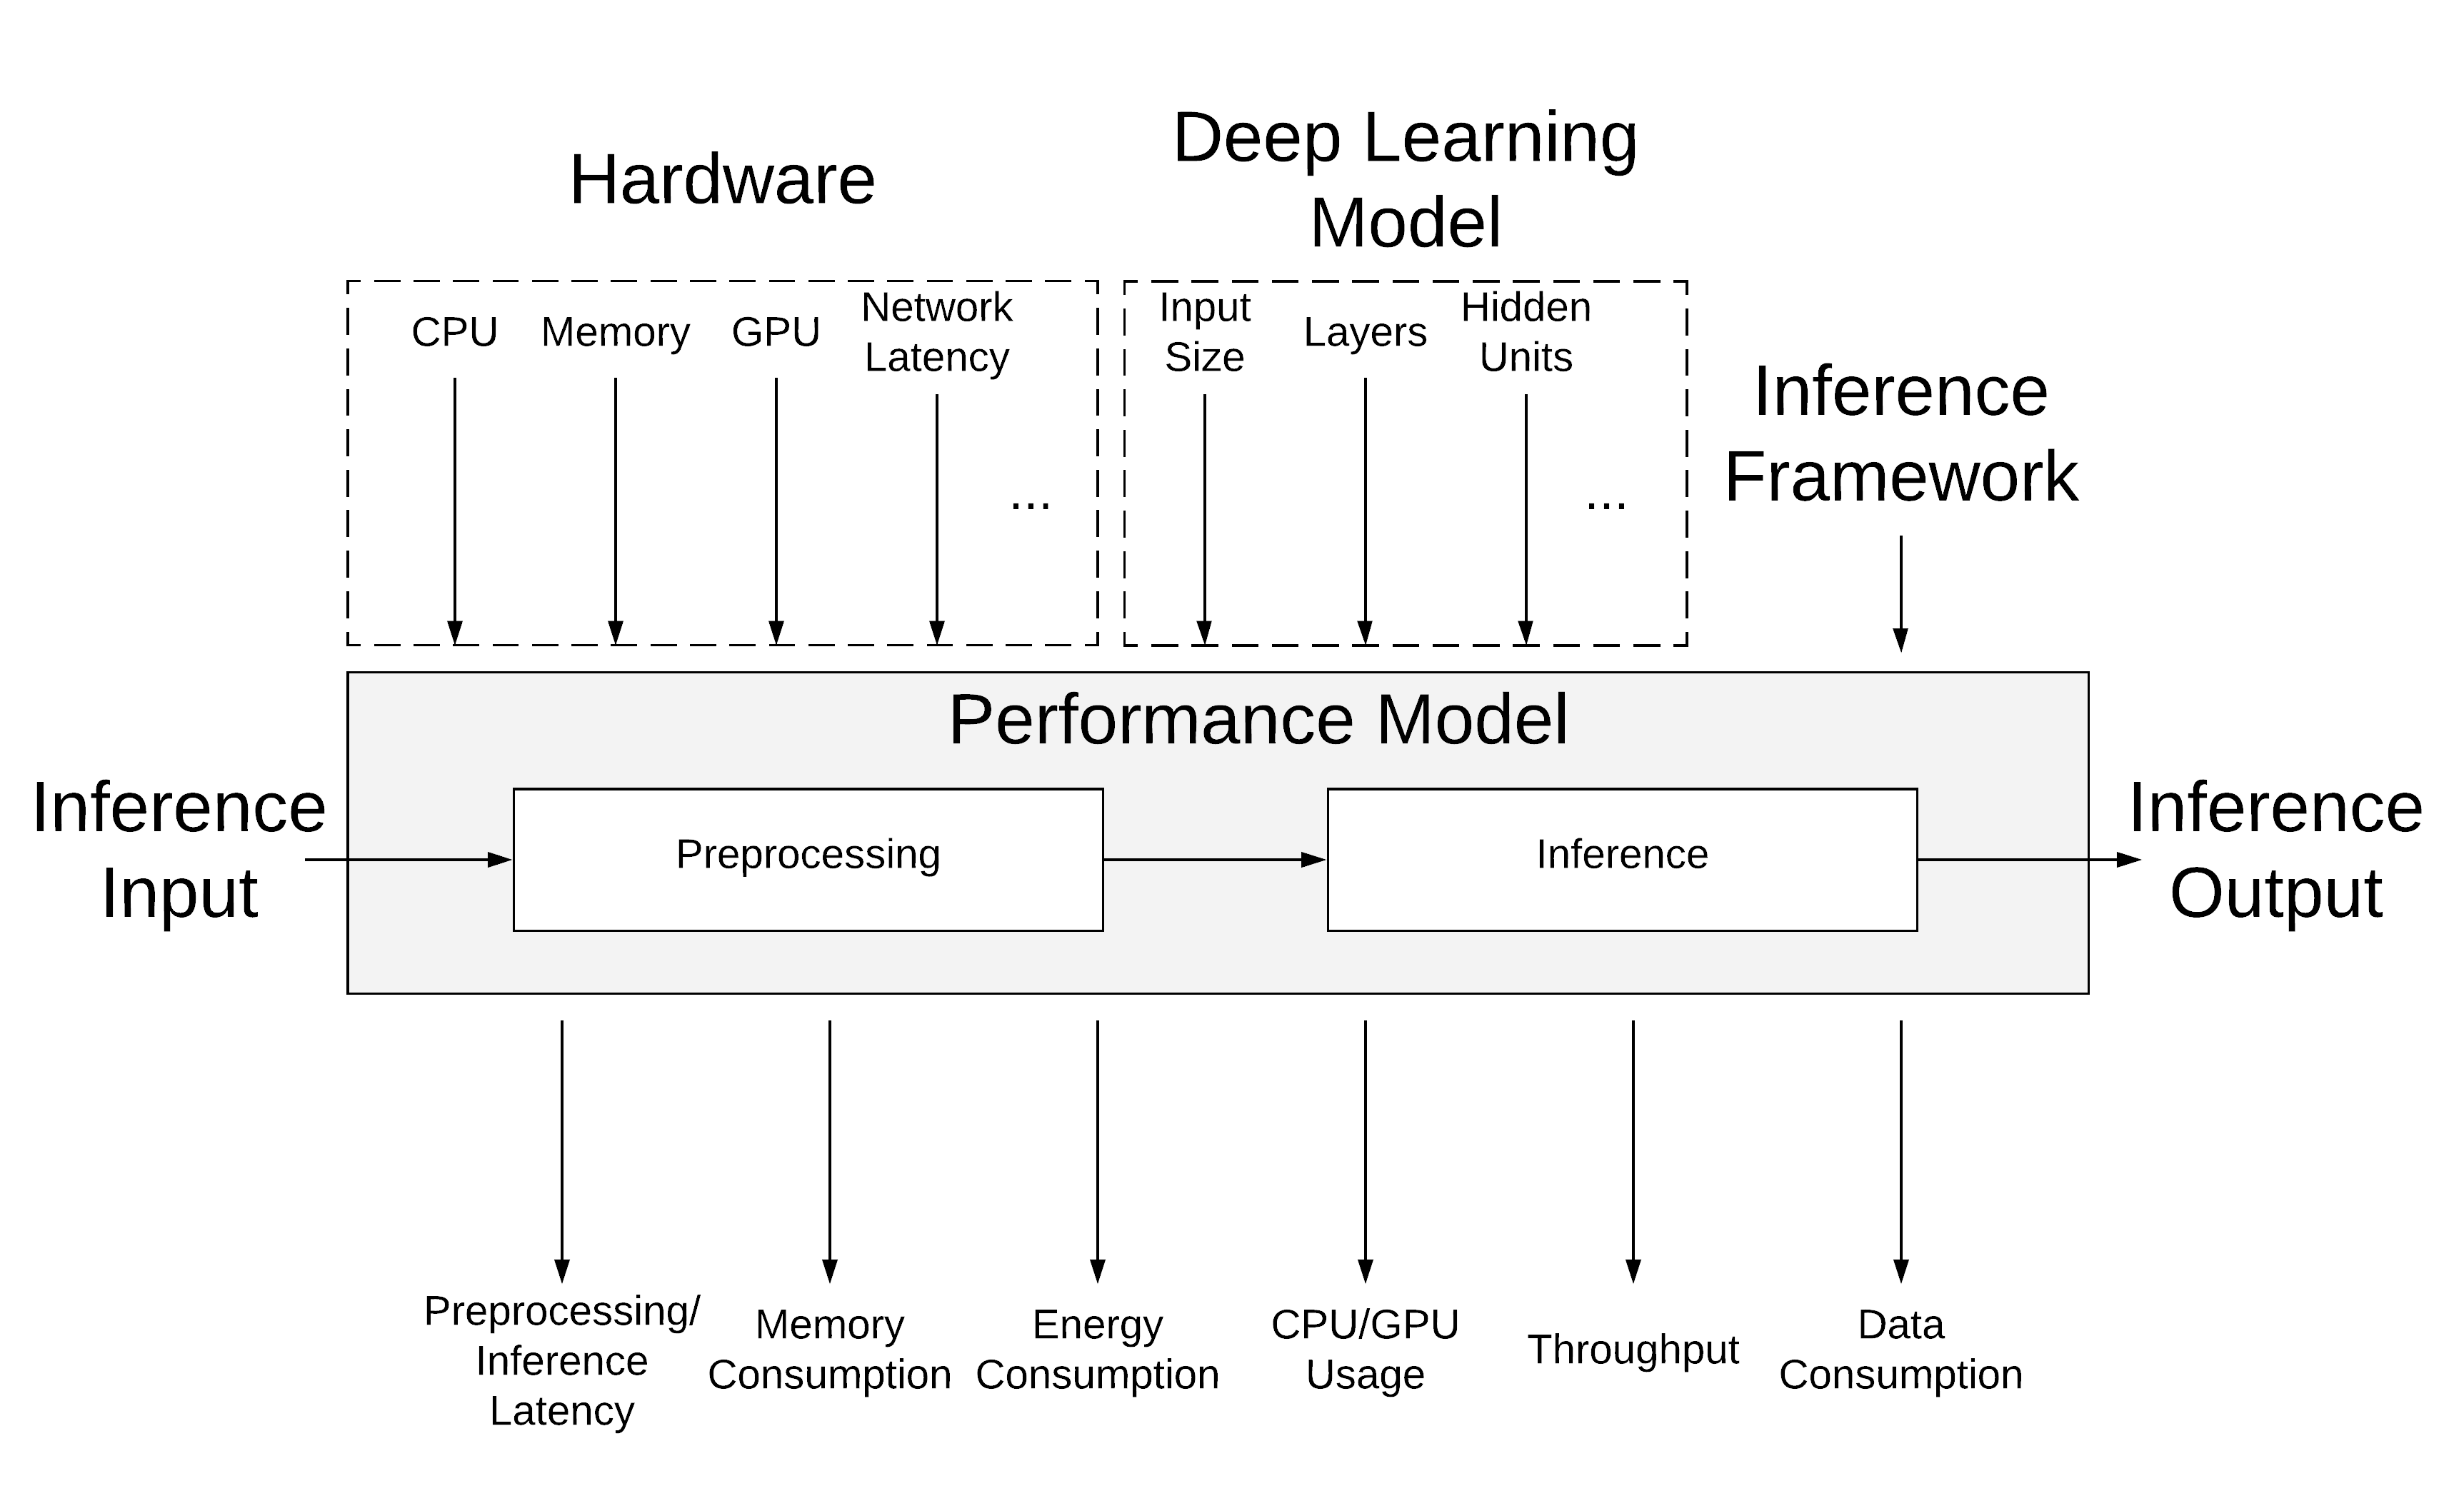
\includegraphics[width=0.99\textwidth]{./Bilder/trade_offs.png}
\caption{Performance Model}
\label{fig:perfmodel}
\end{figure}
\subsection{Performance Metrics}
Several metrics are important to measure the performance of the preprocessing and the inference steps. For the most of the following metrics we break down each metric into two sub-measurements, one for the preprocessing  and the other for the inference part.

\subsubsection{Latency}
Latencies are a essential to determine the performance, since AI application often need predictions in realtime, resulting in the need of low latencies.
The time needed to transform the original input to a shape fit for feeding into the deep learning model is called $Latency_{preprocessing}$.
%%WALL CLOCK TIME ADD HERE
$Latency_{inference}$ describes the time needed from requesting a prediction from a deep learning model given an specific input until getting the prediction.
The latency needed to perform both preprocessing and inference for a given input is called $Latency_{total}$.
\subsubsection{Throughput}
In order to accomplish realtime AI a high enough throughput is essential. Therefore the number of processed predictions per second is a valuable metric. We differentiate between three times of throughput: $Throughput_{preprocessing}$, $Throughput_{inference}$ and $Throughput_{total}$, where the first two are the throughp and the third the throughput for both preprocessing and inference combined.



\subsubsection{Energy Consumption}
$Energy_{preprocessing}$ and $Energy_{inference}$, which describe the amount of energy consumed during preprocessing and inference, are particular important for mobile edge devices, since they often are powered by batteries with a limited lifespan. If the preprocessing or inference process consumes too much energy, the application using the model is not viable.


\subsubsection{CPU/GPU Usage}
Since the preprocessing/inference operations are most of the time not the only processes running on a system and other processes need to run simultaneously to them, the usages of CPU($CPU_{inference}$, $CPU_{preprocessing}$) and GPU($GPU_{inference}$, $GPU_{preprocessing}$) or other available accelerators are an important metric.


\subsubsection{Memory Usage}
Similar to CPU usage, preprocessing and inference should not occupy the whole memory of the system or even demand more memory than the available memory. Therefore $Memory_{inference}$ and $Memory_{preprocessing}$ are of interest.
%\subsubsection{GPU Usage}
%If a GPU or an another accelerator is available their usage is of interest.

\subsubsection{Data Consumption}
$Data_{transmitted}$ and $Data_{received}$ are only relevant for cloud inference, as a request has to be sent to a remote server and the according response with prediction has to be sent back to the client. A high data consumption could slow down the inference latency significantly if the up- and downstream of the network connection is too slow. 

This is in particular important for the case where the input data for the model is preprocessed on the cloud, because the input data is often resized to a smaller shape during preprocessing. Therefore cloud preprocessing increased the amount of data that needs to be transmitted to the server. For slow network connections this could result in higher inference latencies.

%%Add table here?



%%%%%%%%%%%%%%%%%%%%%%%%%%
This section presented the factors influencing the performance of cloud and edge inference and the for the performance significant metrics.
To model the relation between these factors and metrics, we perform experiments on both edge and cloud inference using state of the art hardware, model and framework components. The setup and the result of these experiments are covered in the next section.
\endinput 